\subparagraph*{Submission : }
\textit{Do the same as Step 3 when instead the conversion rate associated with the second item is not known. Also assume that the number of customers per class is not known.}\\

The goal is the same of the previous problem: we have to learn the optimal price for the first item comparing TS and UCB approach. In addition, this time, we have no information about the conversion rate for the second item. 

Implementation: \textit{n4.py}
\subsection*{Strategy}
The script that we have implemented is similar to the previous one. We simulate a random arrival of the customers, proposing the \textit{Racing Skis} to them at the prices suggested by the two learners (UCB and TS) and simulating the purchase of it. In case the customer buys the first item, instead of mathematically retrieve the reward of the second item using the conversion rate, we simulate the purchase of it proposing the \textit{Racing Ski Helmet} at the disconted price accordingly to the user category. We calculate the total reward and we update the learners with the results, as the prevoius submission, normilizing the reward. 

\subparagraph{Implementation} 
\begin{itemize}
	\item No seasonality, conversion rate do no change
	\item The number of customers per class is not known
	\item The conversion rates associated to the second item are not known
	\item Candidates for the \textit{Racing Skis} are: \{2260.0,1910.0,2130.0, 2010.0, 2340.0\}
	\item Conversion rate associated with the first item is not known
	\item Basic price of the Racing Ski Helmet is fixed to 630.0
	\item Promotion assignment is fixed, according to the results of our offline solution: 
	\begin{center}
		\begin{tabular}{ |c|c|c|} 
		\hline
		User category & Assigned promotion & Racing Ski Helmet price \\
		\hline
		Sport Addicted & P$_2$ : 20\% & 504.0 \\
		\hline
		Gifter & P$_1$ : 10\% & 567.0 \\
		\hline
		Amateur & P$_0$ : 0\% & 630.0 \\
		\hline
		Worried & P$_3$ : 30\% & 441.0 \\
		\hline
		\end{tabular}
	\end{center}
	\item Conversion rate associated with the second item is not known
\end{itemize}
\subparagraph{Optimal strategy}
As in the previous submission, the regret is calculated comparing the online approach with an optimal solution. Again, the optimal solution, accordingly to the conversion rate, is to offer the first item at the lower price (1910.0 according to our candidates prices). 

\subsection*{Results}
\begin{center}
	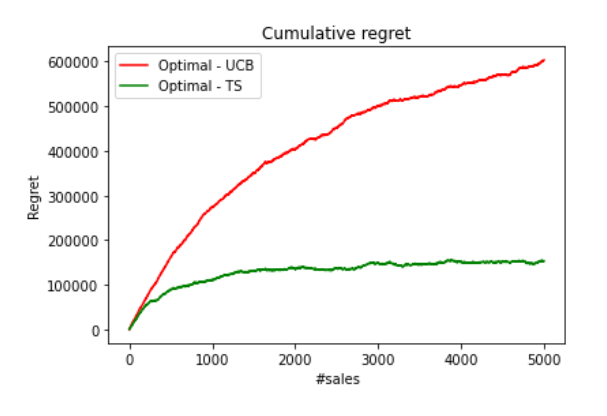
\includegraphics[scale=1.2]{Images/n4}
\end{center}
Days :10\\
Experiments number: 10 \\
Both UCB and TS strategy converge on 1910.0\\
\textit{We have decided to plot the regret of the first 5000 clients, since plotting the results of the entire time horizon made the plot unreadable}

\subsection*{Considerations}
The result shows that a Thompson Sampling approach performs better than a UCB approach, as in the previous problem. The regret curves of both the algorithm are slightly higher than the previous scenario, because, unlike the previous case, we do not know the conversion rates associated to the second item so we have a less precise value that will feed the two leaner, increasing the inaccurancy of the estimations.  
